%!TEX TS-program = Xelatex  
%!TEX encoding = UTF-8 Unicode  
  
  
\documentclass[12pt]{article}  
\usepackage{geometry}  
\geometry{letterpaper}  
  
\usepackage{fancyhdr} 
\usepackage{layout}
\addtolength{\hoffset}{-1.0cm} \addtolength{\textwidth}{2cm}
\addtolength{\voffset}{-1.0cm} \addtolength{\textheight}{2cm}
\usepackage[rgb]{xcolor}

\usepackage{cite}
\makeatletter
\def\@cite#1#2{\textsuperscript{[{#1\if@tempswa , #2\fi}]}}
\makeatother

\usepackage{listings}
\definecolor{dkgreen}{rgb}{0,0.6,0}
\definecolor{gray}{rgb}{0.5,0.5,0.5}
\definecolor{bcol}{rgb}{0.85,0.85,0.85}
\definecolor{mauve}{rgb}{0.58,0,0.82}
\definecolor{mygray}{gray}{.9}
\definecolor{mypink}{rgb}{.99,.91,.95}
\definecolor{mycyan}{cmyk}{.3,0,0,0}
\usepackage{cite} 
\newcommand{\ucite}[1]
{\textsuperscript{\cite{#1}}}

\lstset{ %
language=python,                % the language of the code
basicstyle=\footnotesize,       % the size of the fonts that are used for the code
numbers=left,                   % where to put the line-numbers
numberstyle=\tiny\color{gray},  % the style that is used for the line-numbers
stepnumber=1,                   % the step between two line-numbers. If it's 1, each line
                                % will be numbered
numbersep=5pt,                  % how far the line-numbers are from the code
backgroundcolor=\color{bcol},   % choose the background color. You must add \usepackage{color}
showspaces=false,               % show spaces adding particular underscores
showstringspaces=false,         % underline spaces within strings
showtabs=false,                 % show tabs within strings adding particular underscores
frame=shadowbox,                % adds a frame around the code
rulecolor=\color{black},        % if not set, the frame-color may be changed on line-breaks within not-black text (e.g. commens (green here))
tabsize=2,                      % sets default tabsize to 2 spaces
captionpos=t,                   % sets the caption-position to bottom
breaklines=true,                % sets automatic line breaking
breakatwhitespace=false,        % sets if automatic breaks should only happen at whitespace
title=\lstname,                     % show the filename of files included with \lstinputlisting;
                                    % also try caption instead of title
keywordstyle=\color{blue},          % keyword style
commentstyle=\color{dkgreen},       % comment style
stringstyle=\color{mauve},          % string literal style
escapeinside=``,                    % if you want to add LaTeX within your code
morekeywords={LONG64,LONGLONG,bool}                % if you want to add more keywords to the set
}



\usepackage{flushend, cuted} %

\usepackage{indentfirst,latexsym,bm}
\usepackage{amsmath,amssymb,amsfonts}
\usepackage{pifont} 
\usepackage{fontspec,xltxtra,xunicode}  
\defaultfontfeatures{Mapping=tex-text}  

\usepackage{algorithmic}
\usepackage[noend, ruled, linesnumbered]{algorithm2e}
\setromanfont{华文宋体} %设置中文字体  
\XeTeXlinebreaklocale “zh”  
\XeTeXlinebreakskip = 0pt plus 1pt minus 0.1pt %文章内中文自动换行  
  
 \setlength{\columnsep}{3em}          %设置分栏间隔
\setlength{\parindent}{2em}          %设置段首缩进量
\renewcommand{\baselinestretch}{1.2} %重设行距     
 \usepackage{graphicx}
\usepackage{cite}
\newcommand{\red}[1]{  \textcolor{red}  {#1}}   %红色\makeatletter
\newcommand{\blue}[1]{ \textcolor{blue} {#1}}   %蓝色\def\@cite#1#2{\textsuperscript{[{#1\if@tempswa , #2\fi}]}}
\newcommand{\green}[1]{\textcolor{green}{#1}}   %绿色\makeatother


% ----------------------------------------------------------------
\vfuzz2pt % Don't report over-full v-boxes if over-edge is small
\hfuzz2pt % Don't report over-full h-boxes if over-edge is small

%%--------------------------------------------------
%% 图片文件路径
%%--------------------------------------------------
\graphicspath{{Figures/}}


% MATH -----------------------------------------------------------
\DeclareMathOperator{\diag}{diag}
\DeclareMathOperator{\rank}{rank}
\DeclareMathOperator{\vecm}{vec}
\DeclareMathOperator{\vecs}{vecs}

\newcommand{\mfloor}[1]{ \left\lfloor {#1} \right\rfloor }
\newcommand{\mpair}[2]{ \left\langle {#1}, {#2} \right\rangle}


\renewcommand{\bf}[1]{\mathbf{#1}}
\renewcommand{\vec}[1]{\bm{#1}}    %向量, 黑斜体
\newcommand{\mat}[1]{\bm{#1}}    %矩阵
\newcommand{\dif}{\mathrm{d}}
\newcommand{\me} {\mathrm{e}}
\newcommand{\mi} {\mathrm{i}}
\newcommand{\vei} {\mathrm{vec}}

\newcommand{\vecmat}[1]{\vecm{\left( #1 \right)}}
\newcommand{\vecsmat}[1]{\vecs{\left( #1 \right)}}
\newcommand{\vecasym}[1]{[#1]_\times}   % antisymmetric matrix from a vector
\newcommand{\id} {\mathbbm{1}}   % identity operator
\newcommand{\fracode}[2]{\frac{\dif {#1}}{\dif {#2}}}         % ordinary differential operator
\newcommand{\fracpde}[2]{\frac{\partial {#1}}{\partial {#2}}} % partial differential operator
\newcommand{\fracpderow}[2]{\partial {#1}/\partial {#2}}
\newcommand{\fracoderow}[2]{\dif {#1}/\dif {#2}}
\newcommand{\fracpdemix}[3]{\frac{\partial^2 {#1}}{\partial {#2} \partial {#3}}}
\newcommand{\lap}[2]{\frac{\partial^2 {#1}}{\partial {#2}^2}}
\newcommand{\laprow}[2]{\partial^2 {#1}/\partial {#2}^2}
\newcommand{\secode}[2]{\frac{\dif^2 {#1}}{\dif {#2}^2}}
\newcommand{\set}[1]{\left\{ #1 \right\}}
\newcommand{\abs}[1]{\left| #1 \right|}
\newcommand{\absvec}[1]{\left| \bf{#1} \right|}
\newcommand{\ket}[1]{|#1 \rangle}
\newcommand{\bra}[1]{\langle #1 |}
\newcommand{\braket}[2]{ \langle #1 | #2 \rangle}
\newcommand{\norm}[1]{\lVert #1 \rVert}
\newcommand{\normF}[1]{{\parallel #1 \parallel}_\textrm{F}}
\newcommand{\trsp}[1]{{#1}^\textsf{T}}
\newcommand{\inv}[1]{#1^{-1}}
\newcommand{\ginv}[1]{#1^+}    % Moore-Penrose (general) inverse
\newcommand{\tinv}[1]{{#1}^{-\textsf{T}}}


\newcommand{\ES}[3]{\mathbb{#1}^{{#2}\times {#3}}}               % Euclidean space
\newcommand{\PS}[3]{\mathbb{#1}^{{#2}\times{#3}}}      % projective space
% ----------------------------------------------------------------
\newfontfamily{\H}{微软雅黑}  
\newfontfamily{\E}{Arial}  


\newfontfamily{\TNR}{Times New Roman}  %设定新的字体快捷命令  
\title{{\H Weekly Report of Research Work\\ }\quad {WR-ABS-TEMP-2015A-No.013}}
\author{汤吉(Ji TANG)\\
               Number: WR-ABS-TEMP-2015A,  E-mail: tangji08@hotmail.com \\
        Date: 15/2/2016 - 21/2/2016}
        \date{February 21, 2016}

  
 %%*************************************************
%%  打印 标题, 作者, 日期等内容
%%*************************************************
\begin{document}  
\maketitle
%%*********************************************
%% 设置页眉与页脚
%%*********************************************
\pagestyle{fancy}
\fancyhead[LO,RE]{\leftmark} % clear all fields
\fancyhead[RO,LE]{WR-ABS-TEMP-2015A-No.013-TJx}   %  请设置正确的个人文档编号



\fancyfoot[LO,RE]{SIAE}
\fancyfoot[RO,RE]{Ji Tang}
\renewcommand{\headrulewidth}{0.4pt}
\renewcommand{\footrulewidth}{0.4pt}



%%*************************************************
%% 显示内容目录
%%*************************************************
\tableofcontents 
\newpage
%%*************************************************
%% 正文部分
%%*************************************************
\section{\H Work}
\begin{enumerate}
	\item Reading the book "How to write mathematics ..."
	\item Translating the paper
	\item Studying the R/S method of Feller, Anis and Peter.
	\item Writing the meaning and condition of my project.
	\item Reading a reference paper.
\end{enumerate}

\section{\H The different R/S analysis methods}
For a random series, Feller gave expected $(R/S)_t$ formula
$$E((R/S)_t)=(n*\pi/2)^{0.5}   ~~~~~~~~~(3.1)$$

However, this is an asymptotic relationship and is only valid for large t. Anis and Lloyd provided the following formula to overcome the bias calculated from
(3.1) for small t:
$$E((R/S)_t)=(\Gamma(0.5*(t-1))/(\sqrt{\pi}*\Gamma(0.5*t)))*\Sigma_{r=1}^{t-1}\sqrt{(t-r)/r} ~~~~~~~~~~(3.2)$$

For t>300, it is difficult to calculate the gamma function
by most computers. Using Sterling’s function, formula
(3.2) can be approximated by:
$$E((R/S)_t)=(t*\pi/2)^{-0.50}*\Sigma_{r=1}^{t-1}\sqrt{(t-r)/r}    ~~~~~~~~~~~~~(3.3)$$

Peters gave equation (3.4) as a correction for (3.2)
$$E((R/S)_t)=((t-0.5)/t)*(t*\pi/2)^{-0.50}*\Sigma_{r=1}^{t-1}\sqrt{(t-r)/r}        ~~~~~~~~~~~~~(3.4)$$

\section{\H 课题研究意义}
汇率波动的混沌特性和预测的研究具有以下几个方面的意义:
 
首先,在生产国际化和资本国际化的当今世界经济环境下,加强国际金融特
别是汇率问题的研究具有重要的战略意义。目前,一个国家要增强在国际经济活
动中的能力和应变能力,就必须有畅通的国际金融渠道,这既包括拥有适应本国
经济发展需要的国际支付手段和融资能力,还包括要拥有比较稳定的汇率制度。
而比较完善的、稳定的汇率制度不仅是一国经济发展、财政货币制度的良好反映,
而且对该国的国际经济活动和国际收支调节的顺利进行具有重大影响。所以汇率
问题的研究不论是对国家的宏观经济和微观经济方面,还是在对外经济活动方面
都有十分重要的意义。
 
第二,依照我国经济发展的实际,更需要开展适合我国现有金融体制的汇率
问题研究。随着我国对外开放的不断扩大及我国已加入世界贸易组织,我国的经
济发展和国际经济的联系逐步加强,与国际间的经济交往更加频繁。为了适应瞬
息万变的国际金融市场,我们需要更好地把握国际金融市场的变化和规律,进一
步提高对外汇市场汇率演变预测的准确性,增强对现实汇率变化的阐释能力。
 
种种现象表明,根据目前我国市场经济运行的特点,我国金融市场的演变及
其人民币汇率问题的研究,需要在非线性理论和方法下进行创新,以便对汇率这
一复杂现象作出更为切合实际的描述,从而为我国金融体制的完好运行提供重要
的理论指导,有效地实现对汇率变化特征的阐释和预测。
 
第三,以非线性科学的理论和方法为依据来研究汇率波动的非线性问题是这
一研究的新领域。近年来,随着世界金融市场动荡的加剧,西方的汇率理论对现
实汇率波动规律的解释不同程度的显现出其局限性。汇率波动的复杂性特征进一
步表明了在非线性科学的理论下对传统汇率学说进行理论创新的必要性。因此,
运用混沌和非线性理论与方法来研究汇率波动,是从金融市场的特征性出发来研
究汇率波动的,具有前瞻性和现实性,对提高宏观经济系统运行管理的预见性、
有效性有着重要的理论意义和现实指导意义。
 
第四,汇率预测具有重要的实践应用。汇率无论对国家经济发展、企业经营
及个人投资收益都十分重要。国家、企业及个人都迫切希望能认识汇率行为的规
律。汇率预测的实践应用具有十分重要的意义。就目前最流行的神经网络模型,
具有良好的逼近能力,但由于神经网络的结构过于复杂且难以选择
,
需要估计的
参数相对于较少的数据样本显得太多,导致所得到的神经网络模型相对于数据
容易产生过拟合,泛化能力不够,且具有寻求全局逼近的问题求解方式及收敛速
度慢的缺陷,因而其预测精度不高,在短期汇率预测应用中受到了限制。因此寻
求一种适合短期汇率预测的模型方法具有十分重要的实践意义。
 
\section{\H 汇率预测的研究现状}
对于汇率非线性模型的构建,最流行的方法是神经网络汇率预测模型。早在1993 年,英国的 Refense等人就尝试采用神经网络方法预测汇率变动。近些年来这方面的研究越来越多,并在传统的神经网络预测模型上进行了诸多方面的改进,并取得了较好的预测表现。同时,也出现了许多与神经网络为主的组合预测模型。
 
有关神经网络运用于汇率的实践也开始出现在近期的中文文献中,西安交通大学的魏巍贤和蒋正华
利用神经网络的方法建立了马克/美元汇率短期预测模型,它使用了 1987 年 5 月到 1992 年 12 月 伦敦外汇交易市场和纽约外汇市场马克/美元汇率的周平均数据进行了建模和预测,和传统的线性时间序列模型的预测结果比较,神经网络预测精度高于后者。清华大学的杨忻和马洪波用神经网络预测马克/美元汇率,研究结果表明神经网络比随机游走模型更有效。哈尔滨工业大学管理学院的惠晓峰和胡运权等针对 BP 神经网络所存在的缺陷,结合遗传算法,提出了基于实数编码的 GA-BP 
神经网络汇率预测人民币美元汇率的模型。在结合递归预测方法的基础上,该模型取得了令人满意的结果。
 
神经网络由于具有良好的非线性逼近能力﹑容错性和推广能力,已经在预测
领域广泛应用,但神经网络缺乏可靠的数学表达形式,存在收敛速度慢,结构选
择和局部极小点问题,同时还由于该方法受网络结构复杂度和样本复杂度的影响
较大,因而有时会出现学习或泛化能力过低的现象。

\section{\H A reference paper}
I have read a reference paper which is closely to my project.

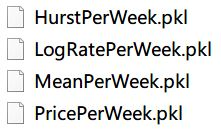
\includegraphics[width=4.5in]{1.jpg}
 

%%****************************************
%%  参考文献
%%****************************************
\bibliography{myreference}
\bibliographystyle{plain}
\end{document}  
